
%% bare_jrnl.tex
%% V1.4b
%% 2015/08/26
%% by Michael Shell
%% see http://www.michaelshell.org/
%% for current contact information.
%%
%% This is a skeleton file demonstrating the use of IEEEtran.cls
%% (requires IEEEtran.cls version 1.8b or later) with an IEEE
%% journal paper.
%%
%% Support sites:
%% http://www.michaelshell.org/tex/ieeetran/
%% http://www.ctan.org/pkg/ieeetran
%% and
%% http://www.ieee.org/

%%*************************************************************************
%% Legal Notice:
%% This code is offered as-is without any warranty either expressed or
%% implied; without even the implied warranty of MERCHANTABILITY or
%% FITNESS FOR A PARTICULAR PURPOSE! 
%% User assumes all risk.
%% In no event shall the IEEE or any contributor to this code be liable for
%% any damages or losses, including, but not limited to, incidental,
%% consequential, or any other damages, resulting from the use or misuse
%% of any information contained here.
%%
%% All comments are the opinions of their respective authors and are not
%% necessarily endorsed by the IEEE.
%%
%% This work is distributed under the LaTeX Project Public License (LPPL)
%% ( http://www.latex-project.org/ ) version 1.3, and may be freely used,
%% distributed and modified. A copy of the LPPL, version 1.3, is included
%% in the base LaTeX documentation of all distributions of LaTeX released
%% 2003/12/01 or later.
%% Retain all contribution notices and credits.
%% ** Modified files should be clearly indicated as such, including  **
%% ** renaming them and changing author support contact information. **
%%*************************************************************************


% *** Authors should verify (and, if needed, correct) their LaTeX system  ***
% *** with the testflow diagnostic prior to trusting their LaTeX platform ***
% *** with production work. The IEEE's font choices and paper sizes can   ***
% *** trigger bugs that do not appear when using other class files.       ***                          ***
% The testflow support page is at:
% http://www.michaelshell.org/tex/testflow/



\documentclass[journal]{IEEEtran}
\usepackage{amsmath}
%
% If IEEEtran.cls has not been installed into the LaTeX system files,
% manually specify the path to it like:
% \documentclass[journal]{../sty/IEEEtran}





% Some very useful LaTeX packages include:
% (uncomment the ones you want to load)


% *** MISC UTILITY PACKAGES ***
%
%\usepackage{ifpdf}
% Heiko Oberdiek's ifpdf.sty is very useful if you need conditional
% compilation based on whether the output is pdf or dvi.
% usage:
% \ifpdf
%   % pdf code
% \else
%   % dvi code
% \fi
% The latest version of ifpdf.sty can be obtained from:
% http://www.ctan.org/pkg/ifpdf
% Also, note that IEEEtran.cls V1.7 and later provides a builtin
% \ifCLASSINFOpdf conditional that works the same way.
% When switching from latex to pdflatex and vice-versa, the compiler may
% have to be run twice to clear warning/error messages.






% *** CITATION PACKAGES ***
%
%\usepackage{cite}
% cite.sty was written by Donald Arseneau
% V1.6 and later of IEEEtran pre-defines the format of the cite.sty package
% \cite{} output to follow that of the IEEE. Loading the cite package will
% result in citation numbers being automatically sorted and properly
% "compressed/ranged". e.g., [1], [9], [2], [7], [5], [6] without using
% cite.sty will become [1], [2], [5]--[7], [9] using cite.sty. cite.sty's
% \cite will automatically add leading space, if needed. Use cite.sty's
% noadjust option (cite.sty V3.8 and later) if you want to turn this off
% such as if a citation ever needs to be enclosed in parenthesis.
% cite.sty is already installed on most LaTeX systems. Be sure and use
% version 5.0 (2009-03-20) and later if using hyperref.sty.
% The latest version can be obtained at:
% http://www.ctan.org/pkg/cite
% The documentation is contained in the cite.sty file itself.






% *** GRAPHICS RELATED PACKAGES ***
%
\ifCLASSINFOpdf
  % \usepackage[pdftex]{graphicx}
  % declare the path(s) where your graphic files are
  % \graphicspath{{../pdf/}{../jpeg/}}
  % and their extensions so you won't have to specify these with
  % every instance of \includegraphics
  % \DeclareGraphicsExtensions{.pdf,.jpeg,.png}
\else
  % or other class option (dvipsone, dvipdf, if not using dvips). graphicx
  % will default to the driver specified in the system graphics.cfg if no
  % driver is specified.
  % \usepackage[dvips]{graphicx}
  % declare the path(s) where your graphic files are
  % \graphicspath{{../eps/}}
  % and their extensions so you won't have to specify these with
  % every instance of \includegraphics
  % \DeclareGraphicsExtensions{.eps}
\fi
% graphicx was written by David Carlisle and Sebastian Rahtz. It is
% required if you want graphics, photos, etc. graphicx.sty is already
% installed on most LaTeX systems. The latest version and documentation
% can be obtained at: 
% http://www.ctan.org/pkg/graphicx
% Another good source of documentation is "Using Imported Graphics in
% LaTeX2e" by Keith Reckdahl which can be found at:
% http://www.ctan.org/pkg/epslatex
%
% latex, and pdflatex in dvi mode, support graphics in encapsulated
% postscript (.eps) format. pdflatex in pdf mode supports graphics
% in .pdf, .jpeg, .png and .mps (metapost) formats. Users should ensure
% that all non-photo figures use a vector format (.eps, .pdf, .mps) and
% not a bitmapped formats (.jpeg, .png). The IEEE frowns on bitmapped formats
% which can result in "jaggedy"/blurry rendering of lines and letters as
% well as large increases in file sizes.
%
% You can find documentation about the pdfTeX application at:
% http://www.tug.org/applications/pdftex





% *** MATH PACKAGES ***
%
%\usepackage{amsmath}
% A popular package from the American Mathematical Society that provides
% many useful and powerful commands for dealing with mathematics.
%
% Note that the amsmath package sets \interdisplaylinepenalty to 10000
% thus preventing page breaks from occurring within multiline equations. Use:
%\interdisplaylinepenalty=2500
% after loading amsmath to restore such page breaks as IEEEtran.cls normally
% does. amsmath.sty is already installed on most LaTeX systems. The latest
% version and documentation can be obtained at:
% http://www.ctan.org/pkg/amsmath





% *** SPECIALIZED LIST PACKAGES ***
%
%\usepackage{algorithmic}
% algorithmic.sty was written by Peter Williams and Rogerio Brito.
% This package provides an algorithmic environment fo describing algorithms.
% You can use the algorithmic environment in-text or within a figure
% environment to provide for a floating algorithm. Do NOT use the algorithm
% floating environment provided by algorithm.sty (by the same authors) or
% algorithm2e.sty (by Christophe Fiorio) as the IEEE does not use dedicated
% algorithm float types and packages that provide these will not provide
% correct IEEE style captions. The latest version and documentation of
% algorithmic.sty can be obtained at:
% http://www.ctan.org/pkg/algorithms
% Also of interest may be the (relatively newer and more customizable)
% algorithmicx.sty package by Szasz Janos:
% http://www.ctan.org/pkg/algorithmicx




% *** ALIGNMENT PACKAGES ***
%
%\usepackage{array}
% Frank Mittelbach's and David Carlisle's array.sty patches and improves
% the standard LaTeX2e array and tabular environments to provide better
% appearance and additional user controls. As the default LaTeX2e table
% generation code is lacking to the point of almost being broken with
% respect to the quality of the end results, all users are strongly
% advised to use an enhanced (at the very least that provided by array.sty)
% set of table tools. array.sty is already installed on most systems. The
% latest version and documentation can be obtained at:
% http://www.ctan.org/pkg/array


% IEEEtran contains the IEEEeqnarray family of commands that can be used to
% generate multiline equations as well as matrices, tables, etc., of high
% quality.




% *** SUBFIGURE PACKAGES ***
%\ifCLASSOPTIONcompsoc
%  \usepackage[caption=false,font=normalsize,labelfont=sf,textfont=sf]{subfig}
%\else
%  \usepackage[caption=false,font=footnotesize]{subfig}
%\fi
% subfig.sty, written by Steven Douglas Cochran, is the modern replacement
% for subfigure.sty, the latter of which is no longer maintained and is
% incompatible with some LaTeX packages including fixltx2e. However,
% subfig.sty requires and automatically loads Axel Sommerfeldt's caption.sty
% which will override IEEEtran.cls' handling of captions and this will result
% in non-IEEE style figure/table captions. To prevent this problem, be sure
% and invoke subfig.sty's "caption=false" package option (available since
% subfig.sty version 1.3, 2005/06/28) as this is will preserve IEEEtran.cls
% handling of captions.
% Note that the Computer Society format requires a larger sans serif font
% than the serif footnote size font used in traditional IEEE formatting
% and thus the need to invoke different subfig.sty package options depending
% on whether compsoc mode has been enabled.
%
% The latest version and documentation of subfig.sty can be obtained at:
% http://www.ctan.org/pkg/subfig




% *** FLOAT PACKAGES ***
%
%\usepackage{fixltx2e}
% fixltx2e, the successor to the earlier fix2col.sty, was written by
% Frank Mittelbach and David Carlisle. This package corrects a few problems
% in the LaTeX2e kernel, the most notable of which is that in current
% LaTeX2e releases, the ordering of single and double column floats is not
% guaranteed to be preserved. Thus, an unpatched LaTeX2e can allow a
% single column figure to be placed prior to an earlier double column
% figure.
% Be aware that LaTeX2e kernels dated 2015 and later have fixltx2e.sty's
% corrections already built into the system in which case a warning will
% be issued if an attempt is made to load fixltx2e.sty as it is no longer
% needed.
% The latest version and documentation can be found at:
% http://www.ctan.org/pkg/fixltx2e


%\usepackage{stfloats}
% stfloats.sty was written by Sigitas Tolusis. This package gives LaTeX2e
% the ability to do double column floats at the bottom of the page as well
% as the top. (e.g., "\begin{figure*}[!b]" is not normally possible in
% LaTeX2e). It also provides a command:
%\fnbelowfloat
% to enable the placement of footnotes below bottom floats (the standard
% LaTeX2e kernel puts them above bottom floats). This is an invasive package
% which rewrites many portions of the LaTeX2e float routines. It may not work
% with other packages that modify the LaTeX2e float routines. The latest
% version and documentation can be obtained at:
% http://www.ctan.org/pkg/stfloats
% Do not use the stfloats baselinefloat ability as the IEEE does not allow
% \baselineskip to stretch. Authors submitting work to the IEEE should note
% that the IEEE rarely uses double column equations and that authors should try
% to avoid such use. Do not be tempted to use the cuted.sty or midfloat.sty
% packages (also by Sigitas Tolusis) as the IEEE does not format its papers in
% such ways.
% Do not attempt to use stfloats with fixltx2e as they are incompatible.
% Instead, use Morten Hogholm'a dblfloatfix which combines the features
% of both fixltx2e and stfloats:
%
% \usepackage{dblfloatfix}
% The latest version can be found at:
% http://www.ctan.org/pkg/dblfloatfix




%\ifCLASSOPTIONcaptionsoff
%  \usepackage[nomarkers]{endfloat}
% \let\MYoriglatexcaption\caption
% \renewcommand{\caption}[2][\relax]{\MYoriglatexcaption[#2]{#2}}
%\fi
% endfloat.sty was written by James Darrell McCauley, Jeff Goldberg and 
% Axel Sommerfeldt. This package may be useful when used in conjunction with 
% IEEEtran.cls'  captionsoff option. Some IEEE journals/societies require that
% submissions have lists of figures/tables at the end of the paper and that
% figures/tables without any captions are placed on a page by themselves at
% the end of the document. If needed, the draftcls IEEEtran class option or
% \CLASSINPUTbaselinestretch interface can be used to increase the line
% spacing as well. Be sure and use the nomarkers option of endfloat to
% prevent endfloat from "marking" where the figures would have been placed
% in the text. The two hack lines of code above are a slight modification of
% that suggested by in the endfloat docs (section 8.4.1) to ensure that
% the full captions always appear in the list of figures/tables - even if
% the user used the short optional argument of \caption[]{}.
% IEEE papers do not typically make use of \caption[]'s optional argument,
% so this should not be an issue. A similar trick can be used to disable
% captions of packages such as subfig.sty that lack options to turn off
% the subcaptions:
% For subfig.sty:
% \let\MYorigsubfloat\subfloat
% \renewcommand{\subfloat}[2][\relax]{\MYorigsubfloat[]{#2}}
% However, the above trick will not work if both optional arguments of
% the \subfloat command are used. Furthermore, there needs to be a
% description of each subfigure *somewhere* and endfloat does not add
% subfigure captions to its list of figures. Thus, the best approach is to
% avoid the use of subfigure captions (many IEEE journals avoid them anyway)
% and instead reference/explain all the subfigures within the main caption.
% The latest version of endfloat.sty and its documentation can obtained at:
% http://www.ctan.org/pkg/endfloat
%
% The IEEEtran \ifCLASSOPTIONcaptionsoff conditional can also be used
% later in the document, say, to conditionally put the References on a 
% page by themselves.




% *** PDF, URL AND HYPERLINK PACKAGES ***
%
%\usepackage{url}
% url.sty was written by Donald Arseneau. It provides better support for
% handling and breaking URLs. url.sty is already installed on most LaTeX
% systems. The latest version and documentation can be obtained at:
% http://www.ctan.org/pkg/url
% Basically, \url{my_url_here}.




% *** Do not adjust lengths that control margins, column widths, etc. ***
% *** Do not use packages that alter fonts (such as pslatex).         ***
% There should be no need to do such things with IEEEtran.cls V1.6 and later.
% (Unless specifically asked to do so by the journal or conference you plan
% to submit to, of course. )


% correct bad hyphenation here
\hyphenation{op-tical net-works semi-conduc-tor}
\usepackage{hyperref}
\usepackage{comment}
\usepackage{graphicx}

% correct bad hyphenation here
\hyphenation{op-tical net-works semi-conduc-tor}

\renewcommand{\vec}[1]{\mathbf{#1}}
\usepackage{amssymb}

%\usepackage{algorithm}
%\usepackage{algorithmic}
\usepackage{url}
\graphicspath{{"D:/PhDWorkwc/PhDWorks/trunk/trunk/CACO/diagrams/"}{"C:/PhDWorks/CACO/diagrams/"}}
%C:/Users/Yang Shi/Dropbox/PhDWorks/trunk/CACO/diagrams/D:/Dropbox/PhDWorks/trunk/CACO/diagrams/

\usepackage[utf8]{inputenc}

\usepackage{listings,lstautogobble}
\usepackage{color}

\definecolor{codegreen}{rgb}{0,0.6,0}
\definecolor{codegray}{rgb}{0.5,0.5,0.5}
\definecolor{codepurple}{rgb}{0.58,0,0.82}
\definecolor{backcolour}{rgb}{0.95,0.95,0.92}

\lstdefinestyle{mystyle}{
	backgroundcolor=\color{backcolour},   
	commentstyle=\color{codegreen},
	keywordstyle=\color{magenta},
	numberstyle=\tiny\color{codegray},
	stringstyle=\color{codepurple},
	basicstyle=\footnotesize,
	breakatwhitespace=false,         
	breaklines=true,                 
	captionpos=b,                    
	keepspaces=true,                 
	numbers=left,                    
	numbersep=5pt,                  
	showspaces=false,                
	showstringspaces=false,
	showtabs=false,                  
	tabsize=2,
	autogobble=true
}

\lstset{style=mystyle}
\usepackage[justification=centering]{caption}
\usepackage{algpseudocode}
\usepackage[]{algorithm2e}
\begin{document}
%
% paper title
% Titles are generally capitalized except for words such as a, an, and, as,
% at, but, by, for, in, nor, of, on, or, the, to and up, which are usually
% not capitalized unless they are the first or last word of the title.
% Linebreaks \\ can be used within to get better formatting as desired.
% Do not put math or special symbols in the title.
\title{Statistical Structural Testing by Continuous Ant Colony Optimization}
%
%
% author names and IEEE memberships
% note positions of commas and nonbreaking spaces ( ~ ) LaTeX will not break
% a structure at a ~ so this keeps an author's name from being broken across
% two lines.
% use \thanks{} to gain access to the first footnote area
% a separate \thanks must be used for each paragraph as LaTeX2e's \thanks
% was not built to handle multiple paragraphs
%

%\author{Yang~Shi,~\IEEEmembership{Portland State University,\\}
 %       X.Song,~\IEEEmembership{Portland State University,}% <-this % stops a space
%\thanks{}% <-this % stops a space
%\thanks{}% <-this % stops a space
%\thanks{}}

% note the % following the last \IEEEmembership and also \thanks - 
% these prevent an unwanted space from occurring between the last author name
% and the end of the author line. i.e., if you had this:
% 
% \author{....lastname \thanks{...} \thanks{...} }
%                     ^------------^------------^----Do not want these spaces!
%
% a space would be appended to the last name and could cause every name on that
% line to be shifted left slightly. This is one of those "LaTeX things". For
% instance, "\textbf{A} \textbf{B}" will typeset as "A B" not "AB". To get
% "AB" then you have to do: "\textbf{A}\textbf{B}"
% \thanks is no different in this regard, so shield the last } of each \thanks
% that ends a line with a % and do not let a space in before the next \thanks.
% Spaces after \IEEEmembership other than the last one are OK (and needed) as
% you are supposed to have spaces between the names. For what it is worth,
% this is a minor point as most people would not even notice if the said evil
% space somehow managed to creep in.



% The paper headers
%\markboth{Journal of \LaTeX\ Class Files,~Vol.~14, No.~8, August~2015}%
%{Shell \MakeLowercase{\textit{et al.}}: Bare Demo of IEEEtran.cls for IEEE Journals}
% The only time the second header will appear is for the odd numbered pages
% after the title page when using the twoside option.
% 
% *** Note that you probably will NOT want to include the author's ***
% *** name in the headers of peer review papers.                   ***
% You can use \ifCLASSOPTIONpeerreview for conditional compilation here if
% you desire.




% If you want to put a publisher's ID mark on the page you can do it like
% this:
%\IEEEpubid{0000--0000/00\$00.00~\copyright~2015 IEEE}
% Remember, if you use this you must call \IEEEpubidadjcol in the second
% column for its text to clear the IEEEpubid mark.



% use for special paper notices
%\IEEEspecialpapernotice{(Invited Paper)}




% make the title area
\maketitle

\begin{abstract}
Statistical software testing plays an important role in software
validation. Automated search for input distributions has been an
effective method to find the near-optimal input distributions for
real-world applications. In this paper, we present an up-to-date
search algorithm based on continuous ant colony optimization (CACO) to
explore effectively the search space for a suitable input
distribution. Our problem formulation decomposes the input
distribution into segments, where each of the segments is dedicated
for a cover element and evolved separately. After the search
termination, all the segments are synergically integrated into one
input distribution. Extensive experimental results demonstrate the
effectiveness and scalability of our approach.
	
	
\end{abstract}

\section{Introduction}
% no \IEEEPARstart
Regression testing plays a very important role in each phase of software development\cite{foundationOfSoftwareTesting}. When a modification is made or a new feature is implemented on the current version of the code base, one needs to perform regression testing to ensure the unchanged code from the new version can continue to work as required. The core problem of regression testing is with regard to the test input selection. In general, the domain of test inputs can be divided into three categories: \(T_r\) is denoted as the regression test set, in which modified version of program needs to be tested to ensure the unchanged functions carried over to the new version are not affected; \(T_o\) is denoted as the obsolete set, in which the test are no longer valid for new version of the program; \(T_u\) is denoted as the redundant set, meaning that a test \(t_u\) in \(T_u\) achieves the same testing objective as a test \(t_r\) in \(T_r\). The test selection problem is to find a minimal subset \(T_r\). In order to find \(T_r\), \(T_o\) should be known in advance. The process of finding \(T_o\) is often referred as \emph{test case revalidation}. This process is dependent on the context of a source code and the test objectives. The process of generating a minimized \(T_r\) is often referred as \emph{test minimization}. In this process, the test entities are often specified in terms of coverage, for instance, branch, statement etc. If more than one test inputs in \(T_r\) can exercise a test entity, then the test input is treated as a redundant test. \emph{Test minimization} aims to form a regression test set \(T_r\) with minimum number of redundant test inputs.

The test set minimization problem can be formulated as the set cover problem\cite{setCoverProblem,foundationOfSoftwareTesting}. Let \(E\) be a set of cover entities, and let \(TE\) be a set of subsets of \(E\), where \(te \in TE\) represents a subset of cover entities exercised by a test input. The test set minimization problem is equivalent to finding a minimum subset \(C \subseteq TE\) that covers all cover items in \(E\). The set cover problem is NP-hard\cite{setCoverProblem}. To solve such problems, approximation methods are commonly used to find the local optimal solution. The use of heuristic algorithms to search for test inputs is widely used in automated test data generation. In \cite{cmimx}, the author uses greedy algorithm to find the minimum covering set. In\cite{branchFunction,branchFunction2,branchFunction3} the concept of \emph{branch function} and \emph{approximation level} are proposed for fitness evaluation. In particular, the \emph{branch function} constructs a continuous fitness landscape for each branch to measure the Euclidean distance of a test input from the critical point of branch execution. The \emph{approximation level} is the number of non-traversable predicates by a searched path corresponding to desired path. The small number of non-traversable predicates indicates that the searched path is closer to the desired path; therefore the fitness of searched path should have a higher value.

%The purpose of testing is to reveal software defects by supplying test input values. In practices, the input domain space can be huge such that it is not possible to test the software by each input. People always want to use a smaller size of test inputs for testing, but achieve higher level of software defection rate so that the testing can be \emph{cost-effective}. However, they are always clueless about the information of faults. Therefore how to select test inputs is a major topic in the area of software testing. Therefore they develop the adequacy criteria of measuring the quality of test set. One of them is called coverage-driven test data generation[] in which the quality of test set depends on the level of coverage reached.

This kind of test data generation approach is called \emph{deterministic structural testing} where the tester selects a priori number of N inputs. The "perfect" cost-effective test set means that each cover element is exercised only once so that the number of inputs are minimized but the number of exercised cover elements are maximized.

However, one question should be asked: will the minimized regression test set have same effectiveness in detecting software faults? For instance, the simple System Under Test (SUT) described in above Figure \ref{fig:SimpleSUT} uses the \(6th\) bit of an input \(x\) to perform a calculation. A careless error caused by a programmer makes the calculation of \(c\) (line 14) incorrect. The simple SUT consists of two branch cover elements: A and B. An input domain space [0, 64] which is separated by A and B into two disjoint subsets: with one ranges from [10, 64] that runs BCE A, and the other one ranges from [1, 9] that runs BCE B. To discover the fault, variable \(b\) must be set to \(1\) so that the test oracle \(c = 3\) mis-matches with \(c\_error = 2\). This infers that only when input \(x\) is equals to \(64\), can the fault be detected.

With this deterministic testing approach, a meta-heuristic search algorithm produces a set of test input aims to reach its branch coverage criteria rather than to reveal the bugs in SUT. In the above example, there are \(54\) choices that can be selected for exercising cover element A, but only one of them can reveal the error. Due to the fact that the number of test inputs for each cover element is fixed, there is no randomness for selecting a test input, which makes it difficult to discover the error similar to the example in Figure \ref{fig:SimpleSUT}.

\begin{figure}
\begin{minipage}{.55\textwidth}
	\begin{lstlisting}[language=c,linewidth=3.8cm, xleftmargin=0.1cm]
	void foo(x)
	{
	
		// x:[0,64]
		
		boolean b = 0;
		int c = 0;
		
		if (x >= 10)
		{
			b = x >> 6 & 1;
			c = b*2 + 1;
			// a human made error. 
			c_error = b + 1; 
		}
	}
	\end{lstlisting}
\end{minipage}
\hspace{0.2cm}
\begin{minipage}{.45\textwidth}
	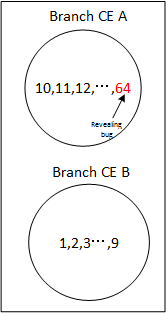
\includegraphics[scale = 0.85]{simplefunc.png}
\end{minipage}
\caption{A simple SUT and its input domain view in terms of branch cover elements}
\label{fig:SimpleSUT}
\end{figure}

Statistical testing generate test inputs by sampling from a probability distribution often called input distribution(input profile) over the input domain space of SUT. Random testing is one of the special cases where the input distribution is uniformly distributed. Duran and Ntafos \cite{evaRandomTesting} evaluated the fault detection performance of random testing by simulation and experimental analysis. Their study showed that random testing can discover some relatively subtle errors without a great deal of effort. In the approach of statistical structural testing, the input distribution needs to guarantee the probability low bound of triggering cover elements by adding the coverage information into the distribution. In above example, suppose the input distribution set the probability low bound of each cover element to \(\frac{1}{2}\), and test inputs inside of each set has equal probability being selected. then the probability of fault discovery by one randomly generated test input is \(p_{(64)} = \frac{1}{2}*\frac{1}{65-10} = 0.91\%\). If we continuously generate samples from input distribution, we could have 99\% confidence that the fault can be detected in \(\frac{1-0.99}{1-0.0091} = 504\) test inputs. 

Construction input distribution encoded with structural information is labor intensive when the size of software increases. Poulding and Clark \cite{searchST} proposed the idea of using meta-heuristic search algorithm to derive optimal/near-optimal distributions automatically. The authors use Bayesian Network as the input distribution model, and Hill Climbing as the search strategy. The authors proposed five hypotheses, and proved each one of them by experiments. Their experiment shows two strong evidences: First, using automated search is able to derive optimal/near-optimal input distributions. Second, input distribution produced by automated search algorithm detect more faults than uniform input distribution. The major problem of their approach is the search-ability. It is difficult for Hill Climbing to escape from the local optima, especially when cover element has separated, disjoint subsets of test inputs and the size of each subset is small. For instance, a cover element \(c_{i}\) has two sub-domains: \(\{x|x \in [1,2]\}\) and  \(\{x|x \in [60,62]\}\). In this case, Hill Climbing is easy to be trapped in the local optima in which only one sub-domain is discovered.

In this paper, in order to solve above optimization problem, we propose another input probability distribution model, and an up-to-date Estimation of Dentition Algorithm (EDA) to optimize this model. Speaking in detail, our contributions are listed in the followings:
\begin{itemize}
	\item We presented a novel approach based on \textbf{C}ontinuous \textbf{A}nt \textbf{C}olony \textbf{O}ptimization algorithm in search-based structural software testing problem.
	\item We created a new input distribution model the \emph{weighted sum of uniform distributions} for test data generation
	\item We analyzed the performance of our approach by running real-world benchmark programs and compared with other search algorithms.
\end{itemize}

The rest of this paper is organized as follows. Section II presents the related work of statistical testing. Section III provides problem formulation of statistical structural testing. Section IV introduces our approach. Section V describes the experimental studies. Section VI draws our conclusions and future work.\\

\section{Related Work}
%Search Based Input distribution Construction
% EDA in Automated Software Testing
\subsection{Search Based input distribution construction}
Traditionally, a search-based algorithm is directly applied to the input domain space, in order to select \(m\) best input vectors with respect to certain coverage criteria. In statistical testing, test data generation is a variation of traditional approaches. The test data are generated with the following steps: First, a search-based algorithm is applied to optimize a probability distribution over the input domain space, to search for an optimal or near-optimal distribution with respect to a certain coverage criteria. Second, A set of input vectors for testing are formed by sampling the input distribution. 

Figure \ref{fig:flow} shows the general framework of search-based input distribution construction. In the initial phase, a uniform or randomly generated distribution is applied to the input domain space. Then a set of test inputs are sampled from the distribution, and seeded into the instrumented SUT and runs. The instrumented code monitors the SUT running status and produces the information of executed traces. Based on the trace information, the fitness value of distribution can be derived by calculating the metric for a specific type of coverages. If the fitness value doesn't satisfy the criteria, the search process is continued in order to refine the input distribution, and to repeat the next iterations until optimal or near-optimal is found. Finally, by sampling the well constructed input distribution, the test data set can be generated.
\begin{figure}[t]
	\hspace*{0.5cm}
	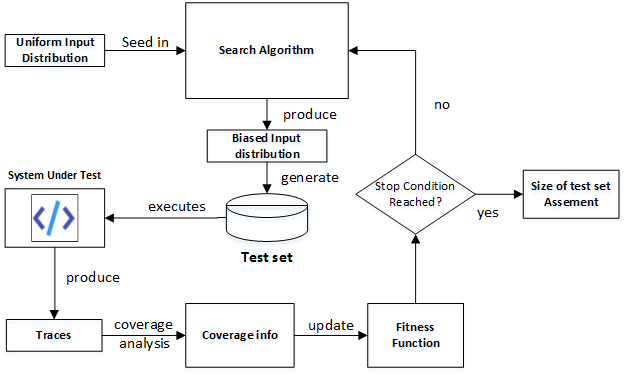
\includegraphics[scale=0.5]{OverallFlow.png}
	\caption{The work-flow of input distribution construction}
	\label{fig:flow}
\end{figure}
\subsection{EDA in Automated Software Testing}
Algorithm \ref{algorithm:1} shows the general process of EDA algorithm. Similar to meta-heuristic algorithms, EDA is given by a initial population of candidates, and output a refined population. The best individual in the final population is the optimized solution. The difference between two approaches is that in EDA, a new population is produced by a probability density function \emph{pdf} which is learned from the highly ranked individuals from the prior population. It is the process of learning the \emph{pdf} function. Once the \emph{pdf} is optimized, it can produce highly fitted individuals for the optimization problem.

\emph{EDA} has been used in software testing problems. Sagarna and Lozano in \cite{eda1} used \emph{MUDA} algorithm to derive a set of test inputs for branch coverage. Ayari, Bouktif and Antoniol in \cite{eda2} applied Ant Colony Optimization to mutation testing problems. Alba and Chicano in \cite{sut} applied evolutionary strategy to evolve a set of test inputs that satisfies the branch coverage.  
\section{Problem Formulation}
In this section, we introduce the concepts of statistical structural testing. 


\begin{algorithm}[t]

	\KwData{A population of candidates}
	\KwResult{An optimized population of candidates }
	Initialize a solution pool with \emph{N} candidates\;
	\While{termination criteria}{
		Select \emph{M} candidates from solution pool according to fitness\;
		Compute the statistics of \(pdf\) model from \emph{M} candidates
		Use the learned \(pdf\) model to generate a new solution pool with \(N\) candidates
	}
	\caption{Generic EDA work-flow}
		\label{algorithm:1}
\end{algorithm}
\subsection{Concept of Statistical Structural Testing}
\subsubsection{Instrumented System Under Test} Let \(D = \{\vec{x}=<x_1,...,x_i,...x_d>|\ L_{i} \leq \vec{x}_i \leq U_{i},\ i = 1, 2, ..., k\}\) be the input domain space of SUT, and let \(C = {\{c_1,c_2 ...c_m\}}\) be the collection of branch cover elements.
Since each test input executes a program path which consists of a collection of branch cover elements,
for each branch cover element \(c_{i}\), there exists a subset \(S_{c_{i}}\) of \(D\) that triggers \(c_{i}\). Formally, we have:
\[S_{c_i} = \{\vec{x}\in D\ |\ \vec{x}\ triggers\ c_{i}\}\]

There exist two types of relations between \(S_{c_i}\) and \(S_{c_j}\) where \(i \neq j\). \(S_{c_i} \cap S_{c_j} \neq \emptyset\) If there exist at least one test inputs trigger both \(c_{i}\) and \(c_{j}\). \(S_{c_i} \cap S_{c_j} = \emptyset\) if no test input can trigger both \(c_{i}\) and \(c_{j}\).\\
\subsubsection{Probability of Triggering a Branch Cover Element}
Let \(P(x)\) be a discrete input distribution. The probability of a test input produced by \(P(x)\) that triggers \(c_{i}\) is:\[\tag{1}\label{eq:ability}p_{c_i} = \sum_{x \in S_{c_i}} P(x)\]

Namely, \(p_{c_{i}}\) is the probability of triggering any one of input vectors inside of \(S_{c_i}\).
In other words, \(p_{c_{i}}\) represents the level of capability of an input distribution to trigger the cover element \(c_{i}\).

\subsubsection{Input distribution Model}
Let \(\vec{x}\) be a test input from input domain space \(D\). Let \(C = \{c_{1},...c_{i},...c_{m}\}\) be the set of branch cover elements. Let \(\{\alpha_{c_{1}},...,\alpha_{c_{i}},...\alpha_{c_{m}}\}\) be a set of mutual exclusive events in which \(\alpha_{c_{i}}\) represents the event of selecting the cover element \(c_{i}\). Then  \(p_{a_{c_{i}}}\) denotes to the desired probability of a sampled test input from the input distribution that covers \(c_{i}\). 
Let the conditional discrete probability \(P(\vec{x}|\alpha_{c_{i}})\) be the probability distribution over input \(\vec{x}\) when the event \(\alpha_{c_{i}}\) occurs.
Then the input distribution \(P(\vec{x})\) is a finite mixture model which is described as follow:
\begin{equation}
\begin{array}{ll}
P(\vec{x}) = \sum_{c\in C}P(\vec{x}|\alpha_{c})p_{\alpha_{c}}\\\\
s.t\  \sum_{i=1}^{m}P_{a_{c_{i}}} = 1
\end{array}
\tag{2}
\end{equation}

The probability of a sampled test input from above settings that triggers cover element \(c_{i}\) is equal to the following equation:
\begin{equation*}
\label{eq:pc}
p(c_{i}) = \sum_{c \in C}\sum_{x \in S_{c_{i}}}P(x|a_{c})p_{a_{c}}
\tag{3}
\end{equation*}

Proof: Let \(P(x,\alpha_{c})\) be the joint probability. Then \(\label{eq:a}P(x,\alpha_{c}) = P(x|a_{c})p_{a_{c}}\). Since \(P(\vec{x}|\alpha_{c})\) is a discrete probability distribution, and for \(\forall \vec{x} \in S_{c_{i}}\ \vec{x}\ triggers \ c_{i}\), \(p(c_{i},\alpha_{c_{i}}) = \sum_{\vec{x} \in S_{c_{i}}}P(x,\alpha_{c=c_{i}})\). Then the total probability \(\label{eq:c}p(c_{i}) = \sum_{c\in C}p(c_{i},\alpha_{c})\). Combining above equations shows the same formula described in equation \ref{eq:pc}.\\

The equation \ref{eq:pc} shows that the actual probability \(p(c_{i})\) is proportional to the desired probability \(p(\alpha_{c_{i}})\). Further more, if \(\sum_{c \in C}\sum_{\vec{x} \in S_{c_{i}}}P(x|a_{c}) \geq 1\), \(p(c_{i}) \geq p(\alpha_{c_{i}})\) . \\
\emph{Theorem:} \(\forall i \in [1,m],\ \sum_{\vec{x} \in S_{c_{i}}}P(\vec{x}|a_{c_{i}})p_{a_{c_{i}}} = 1\) is sufficient for the statement \(p(c_{i}) \geq p_{\alpha_{c_{i}}}\) to be true.\\

\textbf{\small Proof of Sufficiency}: Since \(\sum_{x \in S_{c_{i}}}P(x|a_{c_{i}})p_{a_{c_{i}}} = 1\), 
\(p(c_{i}) = p_{\alpha_{c_{i}}} + \sum_{c_{j}\in C} p(c_{j},\alpha_{c_{j}})\) for \(\forall j \in [1,m], j \neq i\). Therefore, \(p(c_{i}) \geq p_{\alpha_{c_{i}}}\).\\

%\textbf{\small Disproof of Necessary Condition}: Let's suppose in the situation where for \(\forall i,j \in [0, m-1]\land \ i\neq j, S_{c_{i}} \cap S_{c_{j}} \neq \emptyset\). Let the desired probability for each cover element to be \(\frac{1}{m}\). Let \(S_{c_{ij}} = S_{c_{i}} \cap S_{c_{j}}\), and \(\sum_{\vec{x} \in S_{c_{ij}}}P(\vec{x}|c_{j})\) = 1. Since \(p(c_{i}) \geq p_{\alpha_{c_{j}}}*\sum_{\vec{x} \in S_{c_{ij}}}P(\vec{x}|c_{j})\) and \(p_{\alpha_{c_{i}}} = p_{\alpha_{c_{j}}}\),  \(p(c_{i}) \geq p_{\alpha_{c_{i}}}\). Therefore, \(p(c_{i}) \geq p_{\alpha_{c_{i}}}\) is not a necessary condition for statement  \(\sum_{\vec{x} \in S_{c_{i}}}P(x|\alpha_{c_{i}}) = 1\) to be true.\\

The theorem shows that for each one of the conditional probability distributions, if the probability of triggering the targeted branch cover element is equal to \(1\), in the input distribution model, the actual probability of triggering the branch cover element is at least equal to the desired probability. Further more, increasing \(P(\vec{x}|\alpha_{c_{i}})\) can result in the increment of \(p(c_{i})\).

Therefore, how to obtain such conditional probability distributions is the key problem we will solve in the next sections. \\
%The EDA algorithm takes the responsibility to find a set of suitable conditional probability distributions over ttte whole input domain space so that for \(\forall i \in [0,m-1],\ p(c_{i}) \geq P_{\alpha_{c_{i}}}\).\\

\subsubsection {Conditional Probability Distribution Model}
The model of \(p(x|a_{c})\) is chosen to be the \emph{mixture of uniform distributions} (MUD).
The generalized mixture of uniform distributions has the following form:
\[U(\vec{x},\theta_{1},\theta_{2},...,\theta_{n}) = \sum_{i = 1}^{j}\phi_{i}u_{i}(x,\theta_{i*2-1},\theta_{i*2})\]

\begin{figure}[t]
	\hspace*{0.2cm}
	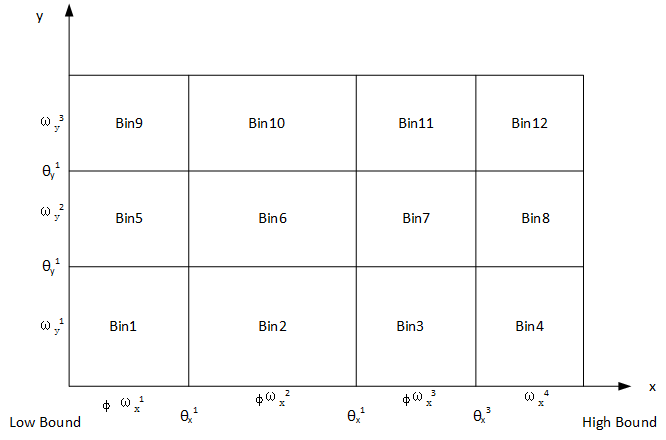
\includegraphics[scale=0.5]{Bin.png}
	\caption{Top view of input domain split by bins}
	\label{fig:bins}
\end{figure}
where \(\phi_{i}\) refers to the weight of i'th component, and the total weight is summed up to \(1\).

\(u_{i}(\vec{x},\theta_{i*2-1},\theta_{i*2})\) represents the i-th component of \(MUD\). It is a multi-dimensional uniform distribution with low bound denoted as \(\theta_{i*2-1}\) and up bound denoted as \(\theta_{i*2}\).\\

In the view of the input domain space, as shown in fig \ref{fig:bins}, \emph{bin} is a fundamental unit to represent a \(MUD\). A \(bin\) is a hypercube which consists of three parameters and both of them are in vector forms: a low limit, an up limit and a weight parameter. The input domain space is separated by a collection of consecutive non-overlapped \(bins\). To sample a test input from the input domain space, we first randomly select a \(bin\) by weight proportionate selection. In what follows, we uniformly pick up a test input from the selected \(bin\).

Mapping from \(bins\) to \(MUD\), the low bound and upper bound can be directly matched. The weight \(\phi_{i}\) of i-th component in \(MUD\) is calculated by the equation in below.

Formally, let \(\vec{\theta}_{i-1}, \ \vec{\theta}_{i}\) denote to the lower limit and upper limit of i-th \(bin\). Let \(\vec{\omega_{i}}\) denotes to the weight of i-th bin. Then the i-th component of \(MUD\) and its weight \(\phi_{i}\) is defined as follow:
\begin{equation}
\begin{array}{ll}
u_{i}(\vec{x},\vec{\theta}_{i-1}, \vec{\theta}_{i}) = \left\{
\begin{array}{rcl}
\frac{1}{|\vec{\theta}_{i} - \vec{\theta}_{i-1}+1|},  \ \vec{x} \in \{\vec{\theta}_{i-1},\ \vec{\theta}_{i}\} \\
0,\ otherwise
\end{array}		
\right. \\
\phi_{i} = \frac{\prod_{d=1}^{dim}\omega_{d}^i}{\sum_{i = 1}^{j} \prod_{d=1}^{dim}\omega_{d}^i}
\end{array}
\tag{4}
\end{equation}
where \(dim\) represents the dimension of the input domain space. \(\phi_{i}\) represents the total weight of the i-th \(bin\). The total weight is the product of weights in each dimension. Each \(\phi_{i}\) is normalized so that all of the weights in \(MUD\) is summed up to 1.

\subsection{Problem Definition}
Constructing the conditional probability distributions by a search method is considered to be an optimization problem. Formally, Let \(C=\{c_{1},...c_{i},...c_{m}\}\) be the set of branch cover elements in side of an SUT. Then for each cover element, a conditional probability distribution needs to be optimized. Let  \(\mathop{U}_{c_{i}}(\vec{x},\theta_{1},\theta_{2},...,\theta_{n})\) be the conditional probability distribution for \(c_{i}\). The optimization problem is defined as follows:
\[\vec{\theta_o} = \mathop{\arg\max}_{\vec{\theta}}\sum_{x \in S_{c_i}} U_{c_{i}}(\vec{x},\theta_{1},\theta_{2},...,\theta_{n}) \]
where \(\vec{\theta_o}\) denotes to a set of optimal parameters. In other words, the objective of optimization is to search for a set of parameters so that the probability of triggering the branch cover element associated to the conditional probability distribution can be maximized.

Calculating \(p_{c_{i}}\) requires to know each test input inside of \(S_{c_{i}}\), and \(S_{c_{i}}\) can only be obtained by exhaustively running SUT over the whole input domain space. Therefore it is necessary to estimate \(p_{c_i}\).

Suppose that the actual probability of a sampled test input triggering \(c_{i}\) is \(p_{*}\), and exactly two outcomes are observed: either sampled test input triggers \(c_{i}\) or it does not trigger \(c_{i}\).
Let \(n_{c_{i}}\) denotes to the number of test input that triggers \(c_{i}\). Suppose \(n\) test inputs are continuously sampled from the input distribution, then the \(n_{c_{i}}\) follows the binomial distribution as follows: 
\[P(n_{c_{i}}) = \binom{n}{n_{c_{i}}}p_{*}^{n_{c_{i}}}\cdot (1-p_{*})^{(n-n_{c_{i}})} \]

By using the maximum likelihood estimation method(MLE) \cite{mle}, the estimated \(p_{c_{i}}\) is derived as follows:
\[ \label{eq:estp}
\tag{5}
\hat{p_{c_i}} = \frac{n_{c_i}}{n}\]

In this paper, both of the experiments conducted on different SUTs use MLE method to estimate the probability of triggering a branch cover element.

%\subsection{Related Work}
%\textbf{{THIS SECTION NOT FINISH}}\\
% Introduction to CACO search methodology, Applied to test data generation(Mutation Testing)
%  Search-based input distribution construction is the key problem of statistical testing. However it is a relative new techniques for test data generation. A representative work is done by Simon and John \cite{statisticaltesting}. They investigated the feasibility and practicality of using automated search algorithm to derive effective input distributions. In their work, Bayesian network is adopted as the distribution model and Hill Climbing method is used as search algorithm. The experimental results proofs that the probability distribution derived using automated search demonstrate the superior efficiency of statistical testing compared to both uniform random and deterministic structural testing.\\

%  Other relevant works about statistical testing are in the followings.


\subsection{Quality of Statistical Test Set} Given an optimal/near-optimal input distribution, the next question is, how many test inputs are good enough to make every cover elements being exercised at least once. Let \(p_*\) be the minimum \(p_{c_{i}}\) among all cover elements. Let \(q\) be the probability of every cover elements can be exercised at least once. Let \(n\) denotes to the size of statistical test set. Then \(q\) is described in the following formula: 
\[\tag{6}\label{eq:testsize}q = 1-(1-p_{*})^n\]

Here \(q\) represents the confidence of triggering the cover element which has the least probability being triggered by \(n\) test input. In the above equation, \((1-p_{*})\) is the probability that a sampled test input does not trigger the cover element. Given \(n\) test inputs, the probability of not triggering the cover element is equal to \((1-p_{*})^n\), from where, we can derive \(q\).\\

To generate test inputs by the search-based statistical testing method, we have two steps:
\begin{enumerate}
	\item \textbf{Searching for a well-suited input distribution}: An efficient search algorithm should be conducted to find the well-suited input distribution. 
	\item \textbf{Determining the size of the test input set}: First, a user should manually decide what confidence level needs to be reached. Second, with given \(p_{*}\) from last step, the size of test inputs \(n\) can be derived from equation \ref{eq:testsize} 
	\[n = \frac{log(1-q)}{log(1-p_{*})}\] 
\end{enumerate}


\section{Our Approach}
\subsection{CACO to Generate Input Distribution}
The use of CACO to optimize the parameters of an input distribution is viewed as a constrained satisfaction problem(CSP) \cite{acocsp}. A CSP is defined as a graph \(G(V,E,C)\) in which \(V \) denotes to a finite set of vertices, \(E\) denotes to the outgoing edges originated from each vertex \(V_{i}\) representing all of the possible values can be assigned to each vertex. \(C\) denotes to a set of the constraints on each vertex. A cost function evaluate the "cost" of selecting a path from the graph. Solving a CSP problem is to minimize the cost function by optimizing the values assigned to each vertex (ie. a path in the graph), at same time, the solution should satisfy the set of constraints.

In our problem, the objective is to optimize the parameters for a set of conditional probability distributions (CPD). Our Optimization problem is defined as follow:

 Let \(k\) denotes to the number of parameters in \(\vec{\theta}\) and \(\vec{\omega}\), and \(\vec{\theta} =\{ \vec{\theta_{1}},...,\vec{\theta_{i}},...,\vec{\theta_{k}}\}\),  \(\vec{\omega} = \{\vec{\omega_{1}},...,\vec{\omega_{i}}...,\vec{\omega_{k}}\}\); Let \([\vec{L},\vec{H}]\) denotes to the input domain space; Let \(dim\) denotes to the dimension of the input domain space; Let \(V_{i}\) denotes to one of the possible assignments in set \(V\) for any parameter; As fig \ref{fig:bins} shows, the number of parameters in \(\vec{\omega}\) is equal to \(k+1\).


For the set of parameters \(\vec{\theta}\), each \(\vec{\theta_{i}}\) in \(\vec{\theta}\) ranges in: \([\vec{L},\vec{H}]\). Therefore the number of outgoing edges from \(\vec{\theta_{i}}\) to \(\vec{\theta_{i+1}}\) is equal to \(||\vec{H}-\vec{L}||_{\mathcal{L}_{2}}\). In order to ensure that there is no overlap between all of the bins that resides in the input domain space, we define the following constraint on \(\vec{\theta_{i}}\) for all \(i\):
\[\forall d \in dim ,\ \theta_{i}[d] > \theta_{i-1}[d]\]
where \(dim\) refers to the dimension of input domain space, \(\theta_{i}[d]\) refers to the d-th component of vector \(\vec{\theta_{i}}\).\\

For the set of parameters \(\vec{\omega}\), let the total weights available for assignment be a constant number \(c\). Let each \(\vec{\omega_{i}}\) in \(\vec{\omega}\) range in: \([0,c]\). Any \(\vec{\omega_{i}}\) in \(\vec{\omega}\) should satisfy the following constraint:
\[\sum_{i=1}^{k+1}\vec{\omega_{i}} = c\]
Since the degree of freedom of above equation is \(k\), the actual number of parameters evolved in optimization is \(k\).

Figure \ref{fig:antGraph} shows the process of distribution construction mechanism. In each iteration, An ant needs to complete a random walk of two cyclic graphs in clockwise rotation. Selecting which edge to be traversed depends on two factors: the amount of pheromone accumulated on the edge, the constraints applied to the corresponding vertex. An edge satisfies the constraint and with higher amount of pheromone accumulated on the edge has a higher probability being chosen. After each ant finishes random walk, a cost function is used to evaluate the "cost" of selecting this path, then \emph{pheromone accumulation} and \emph{pheromone evaporation} functions described in below are performed based on the value of cost. This process is iterated, and the solution is refined at each iteration until a stopping criteria is met.

\emph{pheromone accumulation} and \emph{pheromone evaporation} are the two essential observations of the ants foraging behavior. Describing them in detail:
\begin{itemize}
	\item Pheromone Accumulation. Ants leave pheromone on a path ie, assignment \(V\) of graph \(G\). The amount of pheromone is proportional to the reciprocal of the cost calculated from \(f(A)\). Therefore a more fitted path contains higher amount of pheromone which in turn attracts more ants to walk on the path.
	\item Pheromone Evaporation. The amount of pheromone is decreased with increment of time due to evaporation effect. The time refers to the number of iterations has been finished.
\end{itemize}

Continuous Ant Colony Optimization, simulates the ant foraging behavior, ie. the two pheromone functions by varying the moments of a \emph{Gaussian Distribution} applied to the outgoing edges of each vertex. At initial iteration, the \emph{Gaussian Distribution} has a relative large variance, and the value of parameters are sampled from Gaussian is more random. As iteration increases, the \emph{Gaussian Distribution} is more concentrated such that the value of the parameters has a more fitted mean, and smaller variance.

CACO generalizes its search space from a discrete domain into a continuous domain, which makes it possible to solve real world statistical structural testing problems with a large input domain size. In traditional ACO approach, the solutions are explicitly stored in the memory, which can cause memory explosion problem if the input domain space is too large. With the CACO approach, the solutions are generated from \emph{Gaussian Distributions} which only requires a few bytes to store the parameters of the distributions. %For instance, The \emph{bestmove} SUT contains \(2\) inputs, and each input has a domain size of \(512\). Suppose the number of \(\vec{\theta}\) is equal to \(10\), the the search space for \(\theta\) is equal to  \(512\choose10\). 

\begin{figure}[t]
	\hspace*{0.2cm}
	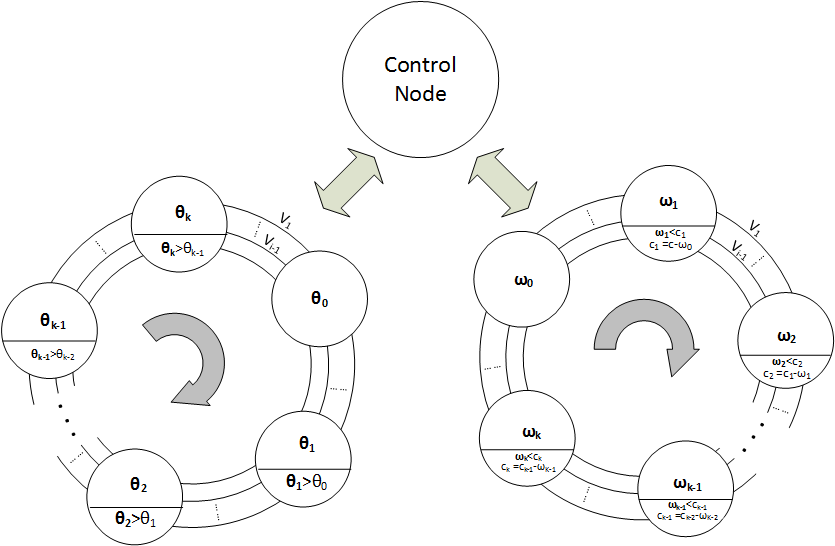
\includegraphics[scale=0.4]{ACO.png}
	\caption{Solution Construction Mechanism}
	\label{fig:antGraph}
\end{figure} 

\subsection{The Whole Process}
The framework of search-based distribution optimization follows standard dynamic testing methodology where the parameter refinement process requires to run SUT during the whole process. Since we evolve each conditional probability distribution(CPD) separately, parallelism implementation is applicable. 

For each CPD, the optimization process begins as follows: At first, a randomly generated pool of solutions are initialized. Next, all of the solutions are ranked by the fitnesses evaluated from the \emph{cost function}. Then for each parameter under the evaluation, a \emph{Gaussian kernel PDF} is learned from the population which encodes the geometric characteristics of the high fitness solutions based on the current population. In what follows, the search algorithm produces a new population of CPDs by sampling the learned \emph{Gaussian kernel PDF}, and then repeats the processes of ranking and evaluation. The search algorithm continues until the search stopping condition is met, Then the best CPD in the population is the optimized solution for the cover element.
\begin{figure}[t]
	\hspace*{0.2cm}
	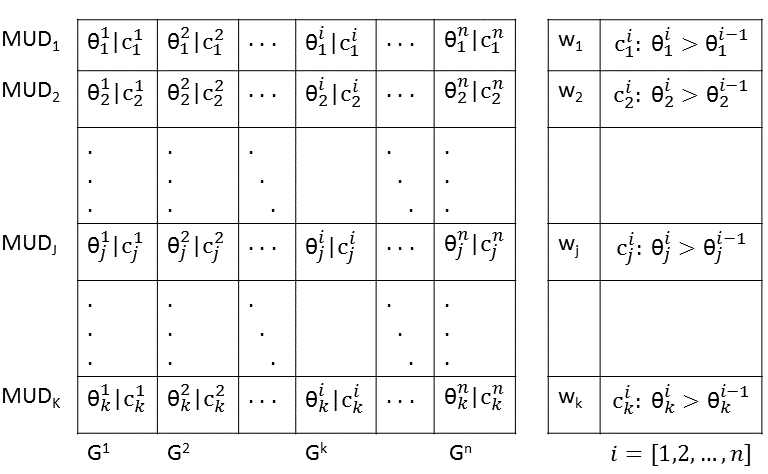
\includegraphics[scale=0.4]{solutionEncoding.png}
	\caption{A representation of partial solution pool for parameter \(\vec{\theta}\)}
	\label{fig:solutionEncoding}
\end{figure} 
\subsection{Encoding of Solutions}
Specifically, Figure \ref {fig:solutionEncoding} represents a population of \(k\) possible configurations of the Mixture Of Uniform Distributions (MUD). The number located in superscript represents the index of a parameter that needs to be optimized; The number in subscript represents the index of a solution in the population. For instance, the value of the i-th parameter in the k-th solution is denoted as  \(\vec{\theta}^i_k\). 

The \emph{Gaussian kernel PDF} used in \emph{CACO} problem is originated from \cite{caco} by Socha and Dorigo. In our problem, Let \(G^{i}\) denotes to the \emph{Gaussian kernel PDF} for i-th parameter. \(G^{i}\) is given by the following equation:
\[G^{i}(\theta^{i}) = \sum_{j = 1}^{n} w_{j}*g_{j}^{i}(\theta^{i})\]
where \(g_{j}^{i}(\theta^{i}) = \mathcal{N}(\mu_{j}^{i},\sigma_{j}^{i^{2}})\) and  \(\omega_{j}\) denotes to the weight associated to the j-th solution. 

In \cite{caco}, the weight of Gaussian component \(g_{j}^{i}(\theta^{i})\) is evaluated by the following equation:
\[w_{j} = \frac{1}{qn\sqrt{2\pi}}e^{-\frac{(l-1)^2}{2q^2n^2}}\] 

where \(l\) denotes to the fitness ranking of l'th UMD, and \(q\) is a preference parameter of the search algorithm. The choice of \(q\) is highly dependent on the specific problem and constraints of the resources. A small \(q\) makes the selection of Gaussian component more biased towards the current best MUD in the population, which could cause the premature convergence problem. A large \(q\) can make the selection to be more uniform distributed, which could increase the possibility of low ranked solutions being selected, and these solutions are hardly to produced a new high fitness solution. 

\(\mu_{j}^{i}\) denotes to the mean of the j-th Gaussian component for i-th parameter. we set the corresponding parameter value in the solution pool as the value of mean, i.e., \(\mu_{j}^{i} = \vec{\theta_{j}^{i}}\)

\(\sigma^{i}_{j}\) denotes to the standard deviation of the j-th Gaussian component for i-th parameter. We apply the same method used in \cite{caco} for updating \(\sigma^{i}_{j}\). The equation is described as follows:
\[\sigma^{i}_{j} = \rho\sum_{k = 1}^{n}\frac{\sqrt{(\theta_{k}^{i} - \theta^{i}_{j})^2}}{n-1}\]

where \(\rho > 0\) is a preference parameter of the search algorithm. The higher value of \(\rho\), the lower convergence speed, but less likely to be trapped in the local optima. It takes the similar effect of conventional ACO algorithm where a large \(\rho\) causes the the pheromone evaporation faster, making the search algorithm difficult to converge.

\subsection{Producing new Solutions}
New solutions are produced by sampling the \emph{Gaussian kernel PDF}. The sampling process takes two steps: First, an index of the Gaussian component in the \emph{Gaussian kernel PDF} (GKF) is randomly generated. Second, in each \emph{GKF}, the Gaussian component with the generated index is used to produce the component of a new solution.
\subsubsection{Generation of Index}
Let \(i\) denotes the i-th component of a GKF. The i-th Gaussian component is selected by the weight proportionate selection method which assigns a probability for selecting each Gaussian component. The equation for probability assignment is defined as follows:
\[P_{i} = \frac{w_{i}}{\sum_{i = 1}^{n} w_{i}}\]
where \(\omega_{i}\) denotes the weight of i-th Gaussian component.
\subsubsection{Constrained Sampling from Gaussian Components}
From Previous step, a set of Gaussian component is given. Let's denote \(\{g^i_1,...,g^i_i,...,g^i_n\}\) as the set of i-th Gaussian components from each \emph{GKF}. Let \(\theta_{i}\) denotes the parameter of the input distribution that needs to be optimized. Each Gaussian component is associated with a constraint, denoted as \(c_{i}\), and \(\theta_{i} > c_{i}\).

Sampling from above settings is equivalent to sampling a truncated Gaussian distribution. Accept-Rejection (AR) sampling is one of the techniques to increase the sampling speed.

Next, we apply AR sampling into our problem:
The constraint \(c^{i}\) of parameter \(\theta^{i}\) can be written as an indicator function \(I(x > c^{i})\) \cite{indicator} such that when \(x > c^{i}\), the function returns \(1\), otherwise it returns \(0\). Then, random variable \(\theta^{i}\) is distributed with the truncated Gaussian distribution defined as below: 
\[\theta^{i} \sim G^{i}(\theta^{i})I(\theta^{i} > c^{i})\]
In AR-Sampling, \(M\) is derived from the following equation
\[M = \sup_{x}\frac{f(x)}{g(x)}\]
where \(f(x)\) represents the truncated Gaussian distribution in standardized form and \(g(x)\) represents the proposed distribution.
In our problem, the truncated Gaussian distribution can be written in the following form:
\[f(x) = N(0,1)*\sigma + \mu\]
and the constraint \(c_{i}\) can be normalized into \(c_{i}^*\):
\[c_{i}^* = \frac{c_{i} - \mu}{\sigma}\]
The the standardized AR sampling can be written as follows:
\[Z_{t} = N(0,1)I(z\geq c_{i}^*)\] 
To derive \(M\) for AR sampling, following equation can be used:
 \[M = \sup_{x}\frac{N(0,1)}{\exp(1) + c_{i}^*}\]

\subsubsection{Fitness Function}
Our search algorithm aims at maximizing the triggering ability \(p_{c_{i}}\) of MUD. Therefore the measure of a MUD adequacy is set to \(p_{c_{i}}\).  As discussed earlier, the value can be estimated by the maximum likelihood method.

\section{Evaluation}
In this section, We evaluate our approach by conducting preliminary experimental studies on two aspects: The performance of search algorithm and the fault detection ability of input distribution for test data generation. We compared the performance of our approach with Hill Climbing, and Genetic Algorithm. We also compared the fault detection ability of the biased input distribution produced by CACO with random testing and deterministic structural testing approaches. We designed our experiments to answer the following research questions:

\textbf{\emph{RQ1: Does CACO performs significant better in searching for the optimal input distribution?}}\\
To answer this question, the following equation is used to evaluate the performance of the derived input distribution for all of the search algorithms which calculates the average probability of triggering all cover elements. The equation is given in the followings:
\[\label{eq:pavg}p_{c_{avg}} =  \frac{1}{|C|}*\sum_{i=1}^{|C|}\frac{n_{c_{i}}}{n}\]
where \(n_{c_{i}}\) denotes to the number of inputs triggers cover element \(c_{i}\); \(n\) denotes to total number of inputs. According to equation \ref{eq:estp}, \(\frac{n_{c_{i}}}{n}\) is the estimated probability of triggering cover element \(c_{i}\).\\
\textbf{\emph{RQ2: Does the input distribution produced by CACO algorithm has a significant increment in detecting software faults than random testing?}}\\
To answer this question, we have evaluated the quality of the test set generated from each distribution by using the mutation testing technique. In mutation testing, a set of mutant versions of SUT was created. A mutated SUT was considered as "killed" if the mutant produces different output from the un-mutated version of SUT or the process was terminated by the operating system. The fault detection ability is measured by the \emph{mutation score}: The proportion of mutants "killed" by a test set. The \emph{equivalent mutant} is allowed to be exists and need not to be identified or removed since our purpose is to compare two test sets.\\
%\textbf{\emph{RQ3: Does the input distribution produced by CACO algorithm has a significant increment in detecting software faults than deterministic structural testing approach?}}\\
%To answer this question, we implemented the Genetic Algorithm to produces a set of test inputs based on the approach created by Tracey, Clark, Mander, and McDermid in \cite{branchFunction}, and used mutation testing for comparing the quality of test sets produced by the two approaches.
\subsection{Experiment Setup}
Four well-known benchmarks are used for experiment analysis. The first test program, \emph{triangleType}, receives three integer numbers as the length of edges in a triangle, and output the triangle type: equilateral, isosceles, scalene, or no triangle. The second test program, \emph{gcd}, receives two integers, and computes the greatest common denominator of the two integer arguments. The third test program, \emph{calday}, computes the day of the week given a date as three integer arguments. The fourth test program, \emph{bestMove}, determines the best move for the current player in a tic-tac-toe game. SUT \(1,2,3\) are adopted from Reference \cite{sut}, and are available at \url{http://tracer.lcc.uma.es/problems/testing/index.html}. SUT \(4\) is adopted from Reference \cite{searchST}, and is available at \url{http://www.cs.york.ac.uk/~smp/supplemental}. The detail characteristics of SUT are shown in the Table \ref{table:1}. %For mutation testing, the mutants are generated from Proteum/IM \cite{proteum}, which is a mutation testing tool for C++ programs.
\begin{table}[t]
\begin{center}
	\begin{tabular}{ |c|c|c|c|c|c|} 
		\hline
		\textbf{Program} & \textbf{Conds.} & \textbf{Args.} & \textbf{Card.} & \textbf{\#tests}  &\textbf{Complexity}\\
		\hline
		triangle & 21 & 3 & 8000 & 200& 2\\ 
		gcd      & 5  & 2 & 2500 & 200  & 1\\ 
		calday   & 11 & 3 & 60000 & 800 & 3\\
		bestmove & 21 & 2 & 262144 & 1000  & 4\\
		\hline
	\end{tabular}
	\caption{Characteristics of SUT}
	\label{table:1}
\end{center}
\end{table}


Producing test inputs by sampling from the distribution follows non-replacement sampling policy, since testing SUT multiple times with same input results in the same output, which is a duplicate work. However in the process of searching for the input distributions, replacement sampling is allowed, since the objective is to maximize the triggering probability of each cover element .

For each SUT, we performed experiments for answering research question 1 and 2 separately. In order to draw a conclusion in a much higher confidence level, we run each experiment for 40 times, and then performed hypotheses testing.

To answer research question \textbf{\emph{RQ2}}, we created the following two hypotheses:

\begin{itemize}
	\item Null hypothesis, \(H0:\) There is no significant difference between fault detection ability within biased input distribution generated from CACO-based approach and that within the uniform distribution.
	\item Alternative hypothesis, \(H1:\) Biased input distribution generated from CACO-based approach can achieve the level of fault detection ability significantly higher than uniform distribution.
\end{itemize}
 
 The experiments are performed in the environment of Windows 10 with 64-bits and runs on Core i7 with 3.5 GHz, 8 logical processors and 16 GB memory. The mutation testing is performed in the environment of Ubuntu 14. 
 
 \begin{figure}[t]
 	\hspace*{0.2cm}
 	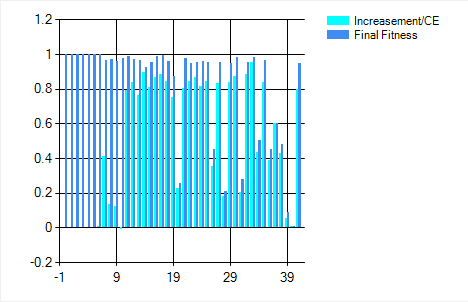
\includegraphics[scale=0.7]{FitnessPerCE.PNG}
 	\caption{The increment on probability low bound over cover elements and the optimized probability low bound}
 	\label{fig:fitnessperce}
 \end{figure} 

\subsection{Result}
\subsubsection{Probability Low Bound}
We estimated the average of the probability low bound for each run, and we compared the result with two other search algorithms: Hill climbing and Genetic Algorithm. Both of the three algorithms shares the same distribution model and the fitness function. We performed experiments on four \emph{SUT} for each of the algorithm. Table \ref{table:2} shows the result of the average estimated probability low bound over the 40 runs. In the table, all of the search algorithms performed well on \emph{gcd}, due to the fact that it is relatively simple and its input domain space is smaller comparing with other \emph{SUT}. As the program complexity increases, \emph{CACO} exhibits the superiority in searching for the optimal input distribution. Fig \ref{fig:cacovs} displays this variation by pairwise comparisons over CACO from data provided in Table \ref{table:2}.\\
Meanwhile, we also take a inside look of the probability low bound of each cover element in the optimization process for the SUT of \emph{bestMove}. We calculate the increment on probability low bound during the optimization process for each cover element and compare them with the optimized probability low bound after the process finishes. Fig \ref{fig:fitnessperce} shows that despite the cover element which has a high probably low bound at the beginning of the optimization process (i.e cover element 1,2,3,4), most of the cover elements are able to be improved by 50\%. However, three cover elements are difficult to be optimized(i.e. 40, 39, 10). This is possibility due to the reason that the inputs that triggers the cover element are either isolated from each other or the size is too small.

 \begin{figure}[t]
	\hspace*{0.2cm}
	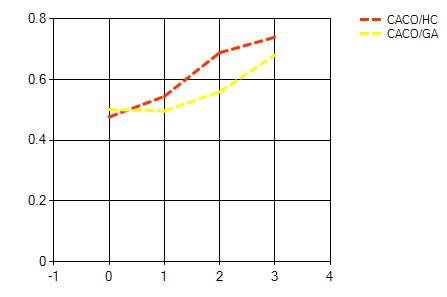
\includegraphics[scale=0.7]{CACOVSOTHER.PNG}
	\caption{CACO exhibits the superiority as complexity increases. X-Axis represents the complexity of SUT; Y-Axis represents the exceeded performance over GA and HC.}
	\label{fig:cacovs}
\end{figure} 

\begin{table}[t]
	\begin{center}
		\begin{tabular}{ |c|c|c|c|c|} 
			\hline
			\textbf{} & \textbf{tri} & \textbf{gcd} & \textbf{calday} & \textbf{bestMove}\\
			\hline
			Hill Climbing & 0.611 & 0.908 & 0.412 & 0.278\\ 
			Genetic Algorithm & 0.742  & 0.986 & 0.716 & 0.460\\ 
			CACO & 0.732 & 0.993 & 0.912 & 0.817\\
			\hline
		\end{tabular}

		\caption{Average of Probability lower bound over
			 40 runs}
		 		\label{table:2}
	\end{center}
\end{table}

 \begin{figure}[t]
	\hspace*{0.2cm}
	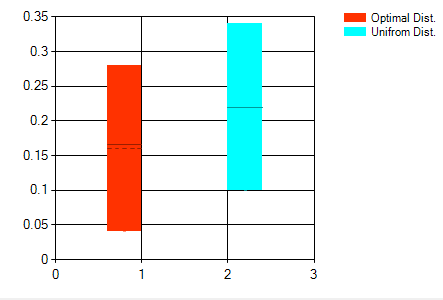
\includegraphics[scale=0.7]{box-gcd.PNG}
	\caption{Mutation Score by uniform distribution and biased input distribution on \emph{gcd}}
	\label{fig:gcd}
\end{figure} 
\begin{figure}[t]
	\hspace*{0.2cm}
	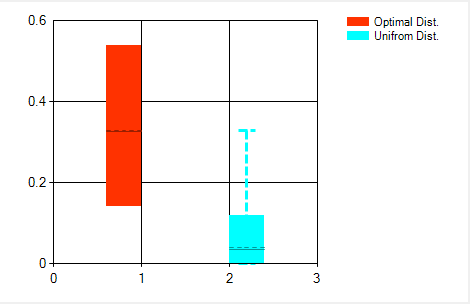
\includegraphics[scale=0.7]{box-bestMove.PNG}
	\caption{Mutation Score by uniform distribution and biased input distribution on \emph{bestMove}}
	\label{fig:bestMove}
\end{figure} 

\subsubsection{Fault Detecting Ability} 
In mutation testing, the original source code is modified by the mutation testing tool which provides a set of mutants of the original SUT. The fault detection ability of the source code depends on how many mutants can be "killed" by the set of test cases. Therefore, the mutation score, which is used to measure the fault detection ability of a test set is defined as follows:
\[Mutation Score = \frac{\#of mutants killed}{total number of mutants}\]

In order to evaluate the fault detection ability, we performed mutation testing 40 times on two SUTs: \emph{bestMove} and \emph{gcd}. for \emph{bestMove}, \(103\) mutants are created, and \(5000\) test cases are sampled from each of the distributions. for \emph{gcd}, \(57\) mutants are created, and \(2000\) test cases are sampled from each of the distributions.
Figure \ref{fig:gcd} and \ref{fig:bestMove} summarizes the experiment result in the form of box plot on \emph{gcd} for both of the two algorithms. These box plots show that the mutation score obtained by uniform distribution is slightly higher than the biased distribution on \emph{gcd}, but significantly lower than biased distribution on \emph{bestMove}. Although in the first experiment, no strong evidents could prove that there is no significant difference between fault detection ability with in two approaches. In the second experiment, the strong evidence proved that biased distribution significantly outperforms uniform distribution by disapproving the null hypothesis. Therefore the second research question is answered. 


 

% For peer review papers, you can put extra information on the cover
% page as needed:
% \ifCLASSOPTIONpeerreview
% \begin{center} \bfseries EDICS Category: 3-BBND \end{center}
% \fi
%
% For peerreview papers, this IEEEtran command inserts a page break and
% creates the second title. It will be ignored for other modes.
\IEEEpeerreviewmaketitle

\section{Conclusion}
Automated statistical structural testing problem is always a challenging problem. It is difficult to derived an optimal input distribution. In this paper we proposed an input distribution model and an up-to-date \emph{EDA} algorithm dedicated to optimize the separated, disjoint and small size sub-domain optimization problems.
Issues of the future work includes the follows:
\begin{enumerate}
	\item \label{i:a1}\textbf{Selection of distribution model:} Input distribution relates to both structure of SUT and the search algorithm. A good input distribution model could reduce the complexity of the search algorithm by setting up the adequate number of parameters in input distribution model and selecting the adequate shape of distributions.
	\item \label{i:a2}\textbf{Selection of search algorithm} The search algorithm itself should have the ability to derive the optimal/near-optimal distribution in reasonable amount of time.
	\item \label{i:a3}\textbf{Estimation of the probability low bound:}  Probability Low bound must be estimated by taking samples from the input distribution. A better estimation method can improve the search efficiency.
	\item \label{i:a4}\textbf{Diversification on test input selection:} The test inputs should be diversified in the entire input domain space, rather than converged to some sub-domain space. However, the probability low bound only gives the probability guarantee over cover elements, rather than the distribution of inputs inside of cover elements. Adding diversification into consideration in the search algorithm could increase the fault detection ability of input distributions.
	\item \label{i:a5}\textbf{Surrogate Model for SUT:} Running SUT consumes physical resources: time, hardware, energy etc. In general, the search algorithm requires to gather coverage information by running SUT in each iteration of the input distribution construction process, which consumes a lot of resources. Building up a surrogate model can help to reduce the amount of time for running SUT by replacing the actual use of running SUT to evaluate the fitness of input distributions.
\end{enumerate}



% if have a single appendix:
%\appendix[Proof of the Zonklar Equations]
% or
%\appendix  % for no appendix heading
% do not use \section anymore after \appendix, only \section*
% is possibly needed

% use appendices with more than one appendix
% then use \section to start each appendix
% you must declare a \section before using any
% \subsection or using \label (\appendices by itself
% starts a section numbered zero.)
%


\appendices
%\section{}
%Appendix one text goes here.

% you can choose not to have a title for an appendix
% if you want by leaving the argument blank
%\section{}
%Appendix two text goes here.

% Can use something like this to put references on a page
% by themselves when using endfloat and the captionsoff option.
\ifCLASSOPTIONcaptionsoff
  \newpage
\fi



% trigger a \newpage just before the given reference
% number - used to balance the columns on the last page
% adjust value as needed - may need to be readjusted if
% the document is modified later
%\IEEEtriggeratref{8}
% The "triggered" command can be changed if desired:
%\IEEEtriggercmd{\enlargethispage{-5in}}

% references section

% can use a bibliography generated by BibTeX as a .bbl file
% BibTeX documentation can be easily obtained at:
% http://mirror.ctan.org/biblio/bibtex/contrib/doc/
% The IEEEtran BibTeX style support page is at:
% http://www.michaelshell.org/tex/ieeetran/bibtex/
%\bibliographystyle{IEEEtran}
% argument is your BibTeX string definitions and bibliography database(s)
%\bibliography{IEEEabrv,../bib/paper}
%
% <OR> manually copy in the resultant .bbl file
% set second argument of \begin to the number of references
% (used to reserve space for the reference number labels box)
\begin{thebibliography}{1}
\bibitem{mle} 
Victor Chew. 
\textit{Point Estimation of the Parameter of the Binomial Distribution}. 
The American Statistician, Vol. 25, No. 5 (Dec., 1971), pp. 47-50.

\bibitem{sut} 
E. Alba and F. Chicano 
\textit{Software Testing with Evolutionary Strategies}. 
In Proceedings of the 2nd Workshop on Rapid Integration of Software Engineering Techniques, Heraklion, Greece, 2005 

\bibitem{muttool} 
M.E. Delamaro and J.C. Maldonado, 
\textit{Proteum/IM 2.0: An Integrated Mutation Testing Environment}. 
Mutation Testing for the New Century, pp. 91-101, Kluwer Academic Publishers, 2001

\bibitem{evaRandomTesting} 
DURAN, J. W. AND NTAFOS, S., 
\textit{An evaluation of random testing}. 
IEEE Trans. Softw. Eng. SE-10, 4 (July), 438–444

\bibitem{searchST} 
Simon Poulding, John A. Clark, 
\textit{Efficient Software Verification: Statistical Testing Using Automated Search}. 
IEEE Transactions on Software Engineering  Volume: 36, Issue: 6, Nov.-Dec. 2010 

\bibitem{branchFunction} 
N. Tracey, J. Clark, K. Mander, and J. McDermid,
\textit{“An Automated Framework for Structural Test-Data Generation”}
Proc. of the 13th International Conference on Automated Software Engineering (ASE’98), Hawaii, 1998, pp. 285-288.

\bibitem{branchFunction2} 
P. McMinn,
\textit{Search-Based Software Test Data Generation: A Survey}
Software Testing, Verification and Reliability, 2004, vol. 14, pp. 105-156.

\bibitem{branchFunction3} 
B. Korel, 
\textit{Automated Software Test Data Generation}
IEEE Transactions on Software Engineering, 1990, vol. 16, no. 8, pp. 870-
879.

\bibitem{setCoverProblem} 
U. Feige., 
\textit{A Threshold of ln n for Approximating Set Cover}
J. of the ACM 45(5): 634–652,1998

\bibitem{foundationOfSoftwareTesting}
Adutta P.Mathur,
\textit{Foundations Of Software Testing 2E}
Pearson

\bibitem{cmimx}
Srivastava P.R., Ray M., Dermoudy J., Kang BH., Kim T.
\textit{Test Case Minimization and Prioritization Using CMIMX Technique}Advances in Software Engineering. ASEA 2009. Communications in Computer and Information Science, vol 59. Springer, Berlin, Heidelberg

\bibitem{aco}
Marco Dorigo, Mauro Birattari, Thomas Stutzle,
\textit{Ant colony optimization}IEEE Computational Intelligence Magazine ( Volume: 1, Issue: 4, Nov. 2006 )

\bibitem{acocsp}
Christine Solnon,
\textit{Ants Can Solve Constraint Satisfaction Problems}IEEE TRANSACTIONS ON EVOLUTIONARY COMPUTATION, VOL. 6, NO. 4, AUGUST 2002

\bibitem{caco}
K. Socha, M. Dorigo
\textit{Ant colony optimization for continuous domains}European Journal of Operational Research 185 (2008) 1155–1173

\bibitem{proteum}
M.E. Delamaro and J.C. Maldonado, 
\textit{"Proteum/IM 2.0: An Integrated Mutation Testing Environment"} 
Mutation Testing for the New Century, pp. 91-101, Kluwer Academic Publishers, 2001.


\bibitem{eda1}
R. Sagarna and J. A. Lozano
\textit{Variable search space for software testing}
International Conference on Neural Networks and Signal Processing, 2003. Proceedings of the 2003, Nanjing, 2003, pp. 575-578 Vol.1.

\bibitem{eda2}
K.Ayari, S.Bouktif and G.Antoniol
\textit{Automatic Mutation Test Input Data Generation via Ant Colony}
GECCO'07, July 7-11, 2007, London, England, United Kingdom

\bibitem{indicator}
Cormen, Thomas H.; Leiserson, Charles E.; Rivest, Ronald L.; Stein, Clifford
\textit{Section 5.2: Indicator random variables}
Introduction to Algorithms(Second ed.). MIT Press and McGraw-Hill. pp. 94–99. ISBN 0-262-03293-7
\end{thebibliography}
\end{document}


